% UNIT: Modeling Concepts
\chapter{Modeling conceptual organization}
\label{chap:modeling_conceptual_organization}

\section[Modeling typicality]{Modeling typicality\\ \large{\textit{Deep Neural Networks Predict Category Typicality Ratings for Images}\\ \mandatory{lake-2015-deep}}}

They evaluate deep convolutional networks trained for classification on their ability to \textbf{predict category typicality} (human typicality ratings), and try to understand whether deep learning systems can serve as potential cognitive models.

\subsection{Background}
The motivation is that, for any task that requires relating an item to its category, \textbf{typicality will influence performance}, whether it is the speed of categorization, ease of production, ease of learning, usefulness for inductive inference, or word order in language.

CNNs learn categorization, but \textbf{perhaps they categorize by learning prototypes}, i.e., they produce representations that track categorical structure with typicality structure.

\subsection{Methods}
They asked people to rate a collection of images for category typicality (images drawn from 8 image categories), and tested different CNN architectures on their ability to predict these ratings.

\subsubsection{Behavioral experiment}
Each participant rates ``how well does this picture fit your idea or image of the category". Mean typicality per image is computed across all splits. Human reliability ratings have good split-half correlation: the average reliability of human ratings across random splits is $\rho=0.92$. This confirms that two groups of people produce similar rankings \notet.

\osst{This is required to know if we can trust human ratings (i.e. \textit{is human behaviour reliable enough to predict itself?}). If we could not trust human data, there would be no point in aligning the model output to human ratings.}

\subsubsection{Computational experiment}
They use 3 CNN architectures (but for the sake of simplicity \textit{OverDeat} only is described). After the convolutions, the next two layers have 3072 and 4096 fully-connected units, respectively.
Finally, a 1000-way softmax layer produces a probability distribution over the $j = 1,\dots,1000$ classes. They get a top-five error rate of 14.2\% \notet.

\osst{Top-five error: the correct label did not appear in the top five guesses.}

\subsection{Estimating image-typicality}
They assume that (human) \textbf{typicality is related to the strength of the model’s classification response} to the category of interest.
The \textbf{classification strength} can be estimated in two ways:
\begin{itemize}
    \item \textbf{Raw typicality}: This is a raw category score. There is a theoretical vector (input of last layer) which \textbf{maximizes the activation} of a particular category. Images with representation very close to this theoretical vector are expected to be more typical. So we can maximize $y_j$ to get the particular abstract representation for each category $j$:
    \[
    y_j = \sum_{i=1}^{4096} w_{ij}x_i
    \]
    \item \textbf{Contrast typicality}: It measures to what extent the correct category is more active than the others. It benefits images that load on the correct category much more than on other ones. The most typical image produces $y_j$ that is most differentiated from other categories’ response to this image. This is independent from the raw value:
    \[
    z_j = \frac{e^{y_j}}{ \sum_{j=1}^{1000} e^{y_j} }
    \]
\end{itemize}

The values computed for each $j$ are averaged, then they check for correlation with human ratings.

\subsection{Results}
\begin{wrapfigure}[16]{r}{0pt}
  \centering
  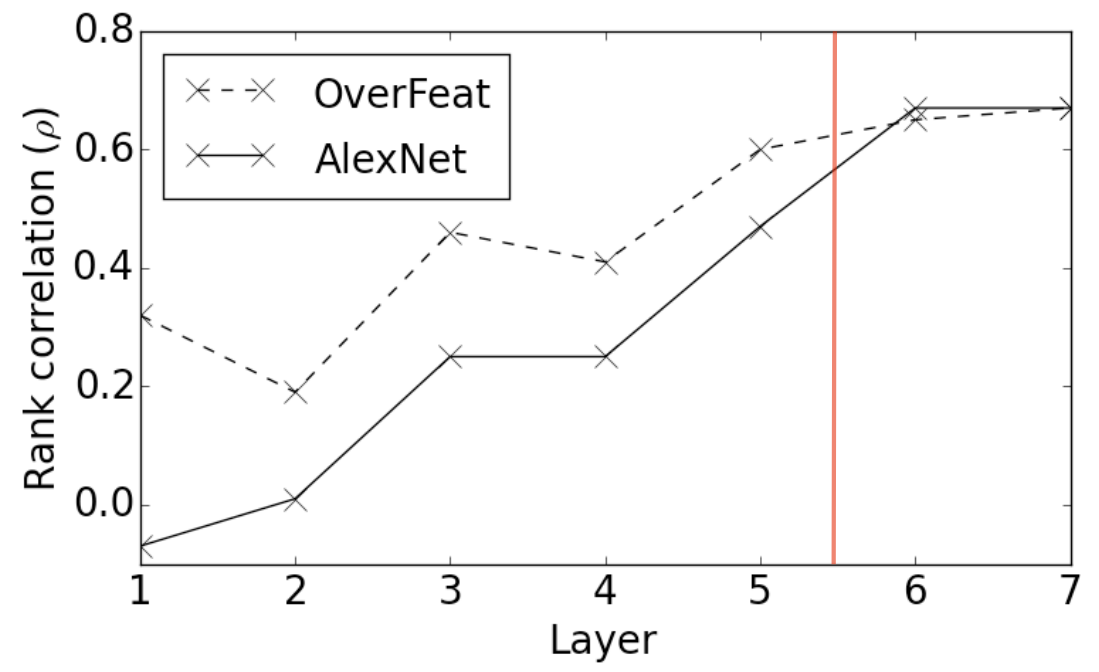
\includegraphics[width=0.4\textwidth]{images/lake.png}
  \caption{Correlation between human and convnet typicality ratings as a function of network depth. The red line indicates a transition from convolutional (1-5) to standard layers (6-7).}
  \label{fig:lake}
\end{wrapfigure}

They found that raw and contrast scores do similarly well, and that some models have significant human-machine typicality correlation. This suggests that deep \textbf{CNNs learn graded categories that can predict human typicality ratings}, at least for some types of everyday categories.\\

However, when dealing with hidden layers, one cannot have categories' activations, so they needed to redefine typicality.
They used 1300 images (of the same category) as input for the network and averaged the activation of the given layer over all images to get the \textbf{category prototype} (typical activation vector).
Typicality was modeled as the cosine distance between the activation vector for a new image and the stored prototype. They found better prediction in deeper convolutional layers (see Figure~\ref{fig:lake}), i.e., by going deeper (closer to the output layer) the layer representations predict increasingly better human typicality.


\section[Words-as-features as models of cognition]{Words-as-features as models of cognition\\ \large{\textit{Predicting Human Brain Activity Associated with the Meanings of Nouns}\\ \mandatory{Mitchell2008PredictingHB}}}
They try to answer this question: Can feature models explain behavioral and brain responses?
The underlying idea is to understand how/where word meaning is stored in the brain, under the assumption that our brain represents words as features. Notice: this assumption is not necessarily true, there might be also other possibilities (not tackled in this paper).

\subsection{Background}
Core questions for neuroscience are:
\begin{itemize}
    \item Are there systematic differences in neural activity as people think about different concepts? 
    \item Is the neural representation of concepts localized in specific brain areas or is it distributed across the entire cortex?
    \item How meaningful are individual differences, or is the \textit{representation of meaning} similar across people?
\end{itemize}

We ask ourselves if fMRI and neuroscience allow us to \textit{test} or \textit{understand} what are the \textbf{basis functions} (the \textbf{semantic feature} space) that underlie the representation of words. This can help in designing more cognitive real computational models.

\boxc{Historical approach}{
We present multiple words sampled from several categories (e.g. tools, buildings), and then train a classifier that predicts the class (tool/building) from the brain images of the words. Brain images are taken with fMRI: see the figure, which shows activation maps from fMRI data (each of the 4 images in a row represent a slice of the brain). A classifier can be trained using a single voxel.
The results of the classifier can be used as a tool for studying the semantics in the brain. For instance, we can understand which brain area contains information about particular classes. This is a pure \textit{decoder}; there is no domain-based knowledge that is applied to predict the brain response from more basic principles.

\begin{center}
    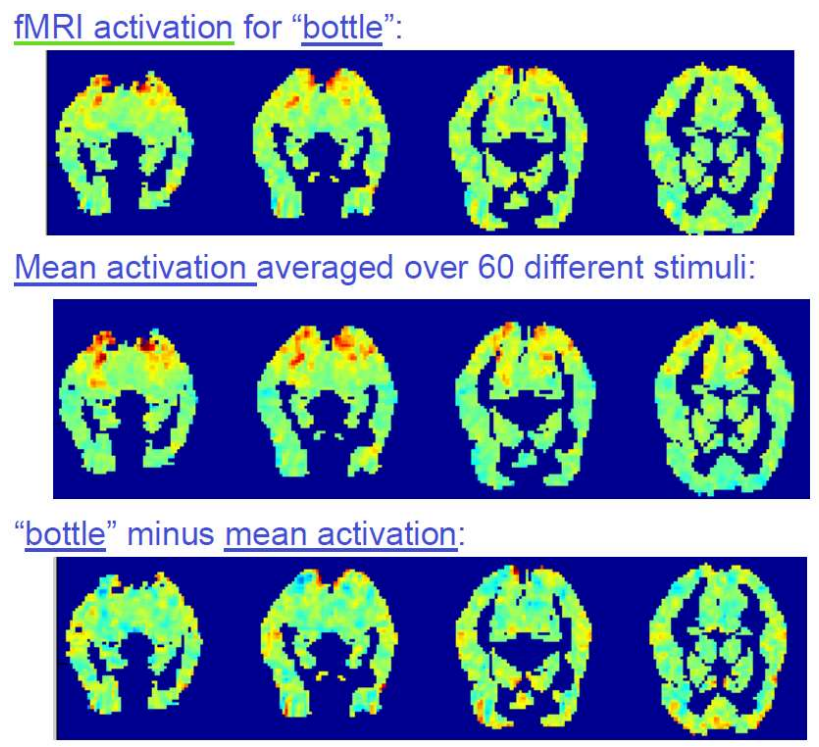
\includegraphics[width=0.5\textwidth]{images/fmri_slices.png}
\end{center}

Classifiers capture some meaning, as they show \textbf{cross-domain generalization} (train on words, guess class of image).
They collected brain activity while people watched an image (instead of the word), and while Portuguese (instead of English) people watched the same words.
They then took the classifier trained to discriminate categories based on brain responses to words presented in English and tested on brain activity from those other domains. 
Both \textit{testing on pictures} and \textit{testing on other language} produce above chance accuracy: \textbf{semantics generalize beyond modality used}.
}

The historical (decoding) approach works, but has a problem: \textbf{data is highly dimensional} (over 20 thousand features/voxels per word). At the same time, however, \textbf{data is also sparse} (only few examples of brain activity per category). This is difficult from a regression perspective and solutions to this (regularization) are mathematically valid but may lose information about the brain.
These considerations sparked \cite{Mitchell2008PredictingHB} to propose an alternative.

\subsection{Generative encoding model}
\begin{wrapfigure}[13]{r}{0pt}
  \centering
  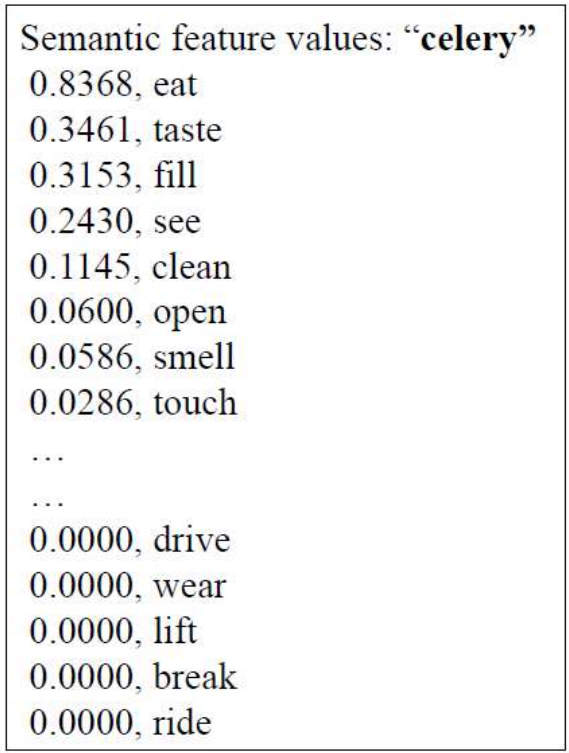
\includegraphics[width=0.23\textwidth]{images/mitchell_2.png}
  \caption{Example of feature vector.}
  \label{fig:mitchell_2}
\end{wrapfigure}
Their proposal is to \textbf{come up with a theory of word meaning and see whether the theory predicts brain activity} (\textit{activation}). They capture ``word meaning" from corpus statistics (from mutual constraints appearing in corpora). The challenge is basically to find a ``mapping function" from word meaning to brain activity.
\begin{figure}
    \centering
    \captionsetup{width=.8\linewidth}
    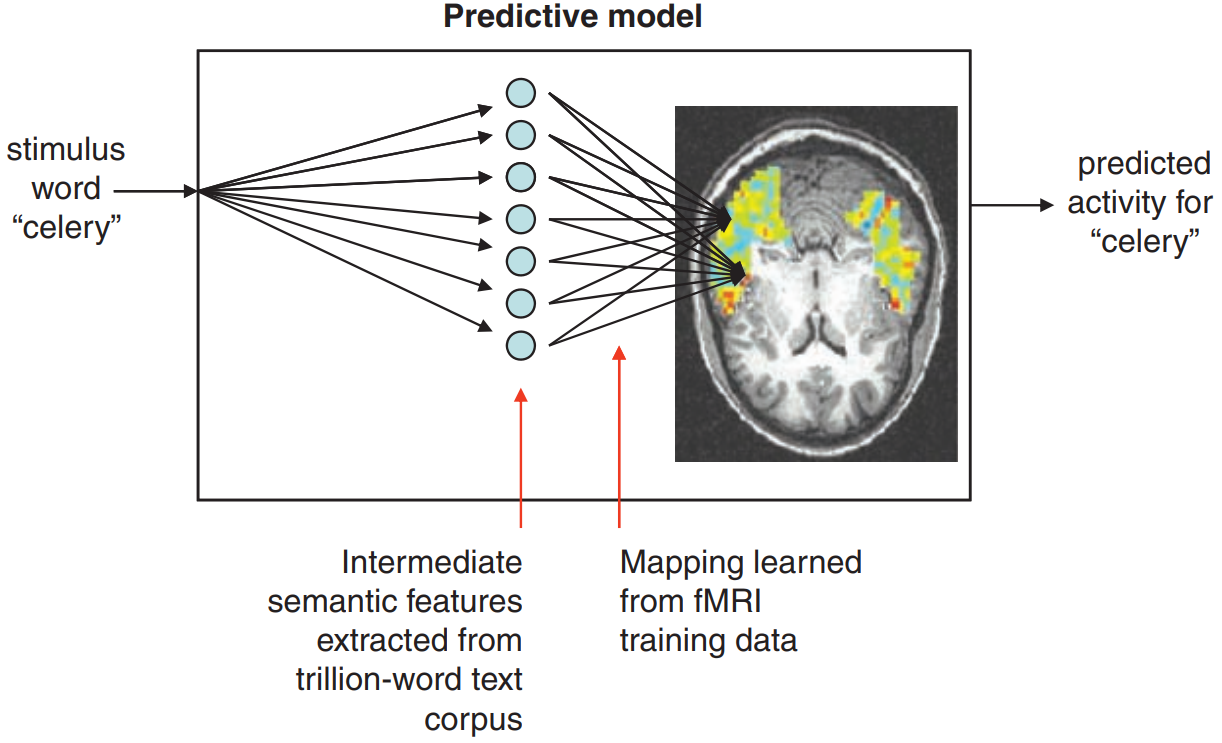
\includegraphics[width=0.55\linewidth]{images/mitchell.png}
    \caption{The predictive encoding model. Each word gets a vector of $n$ features (in this simplified schema just 7); the value of $n$ has to be chosen as it is a hyper-parameter. Note: there is no single step prediction for the whole brain. The prediction is done for a single pixel, i.e., we get a weight vector for each voxel. Then all pixels are put together to get the whole map.}
    \label{fig:mitchell}
\end{figure}

The model works in two steps. The first step encodes the stimulus word.
The second step predicts the neural fMRI activation at every voxel location in the brain, as a weighted sum of neural activations contributed by each of the intermediate semantic features. A schematic explanation can be seen in Figure \ref{fig:mitchell}.

\subsubsection{Define word meaning}
We mentioned that they captured word meanings via corpora exploitation. They use 60 \textbf{nouns}. Each noun $j$ is described using 25 \textbf{features}.\\
Feature $i$ is defined as the \textbf{co-occurrence frequency of the stimulus noun with the verb} $i$. They chose verbs which are either: \textit{sensory}, \textit{motor}, or \textit{abstract} verbs. An example of the resulting semantic features is provided in Figure \ref{fig:mitchell_2}.

\subsubsection{Single-voxel analysis}
They perform a single-voxel analysis. For each voxel in the brain they learn the relation between voxel activity values for the 60 nouns, and the semantic features of the 60 nouns \notet.

Such analysis can tell, \textbf{for each voxel},\textbf{ what is the relative importance of each of the 25 features} when it comes to predicting brain activation. To show generalization, they train the model with 58 words and test on the remaining 2.

In matrix notation the multiple regression model is $\mathbf{Y=X}\boldsymbol{\beta}+\boldsymbol{\varepsilon}$, where:
\[ 
     \mathbf{Y} = \begin{bmatrix}
     Y_1 \\ Y_2 \\ \vdots \\ Y_n
     \end{bmatrix}, \quad\; 
     \boldsymbol{\varepsilon} = \begin{bmatrix}
     \varepsilon_1 \\ \varepsilon_2 \\ \vdots \\ \varepsilon_n
     \end{bmatrix}, \quad\;
     \boldsymbol{\beta} = \begin{bmatrix}
     \beta_0 \\ \beta_1 \\ \vdots \\ \beta_k
     \end{bmatrix}, \quad\;
     \mathbf{X} = \begin{bmatrix}
     1 & X_{11} & \dots & X_{1k}\\
     1 & X_{21} & \dots & X_{2k}\\
     \vdots & \vdots & \ddots & \vdots\\
     1 & X_{n1} & \dots & X_{nk}\\
     \end{bmatrix}
\] 
$\mathbf{Y}$ is the activity for the 58 nouns in the voxel; $\boldsymbol{\varepsilon}$ is the bias; $\boldsymbol{\beta}$ are the 25 weights to be fit; $\mathbf{X}$ is the set of 25 feature-value per noun ($n=25, k=58)$.

\osst{To be precise, they present stimuli of noun+image together (but for the sake of simplicity we refer to them just as ``nouns").}

Predicting word activity in each voxel just means multiplying its semantic feature values by learned weights (Figure \ref{fig:mitchell_3}).
\begin{figure}[!ht]
    \centering
    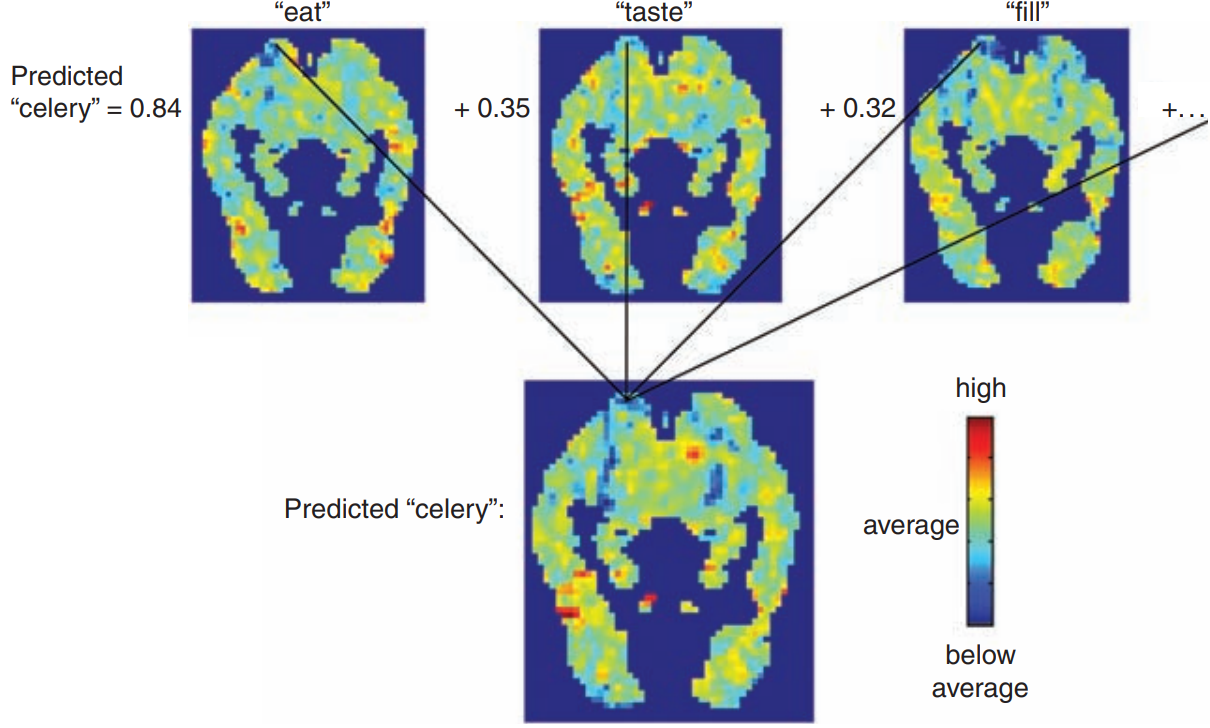
\includegraphics[width=0.6\linewidth]{images/mitchell_3.png}
    \caption{Predicting fMRI image for given word.}
    \label{fig:mitchell_3}
\end{figure}

\subsection{Results}
They tested the model by predicting activity for word A, and checking if it is more similar to true activity of word A than it is to the other word B (where A and B are the two left over words, not used for training). They got an average accuracy of 0.79, suggesting that word meanings are indeed \textbf{represented as features in the brain}.\\

They also examined, for each of the 25 features (verbs), the importance across the brain, to obtain a map of which brain areas are the most important for a given verb (and therefore for a given activity, see Figure \ref{fig:mitchell_4}).\\

\begin{figure}[!ht]
    \centering
    \captionsetup{width=.8\linewidth}
    \begin{subfigure}{.52\textwidth}
        \centering
        \captionsetup{width=.8\linewidth}
        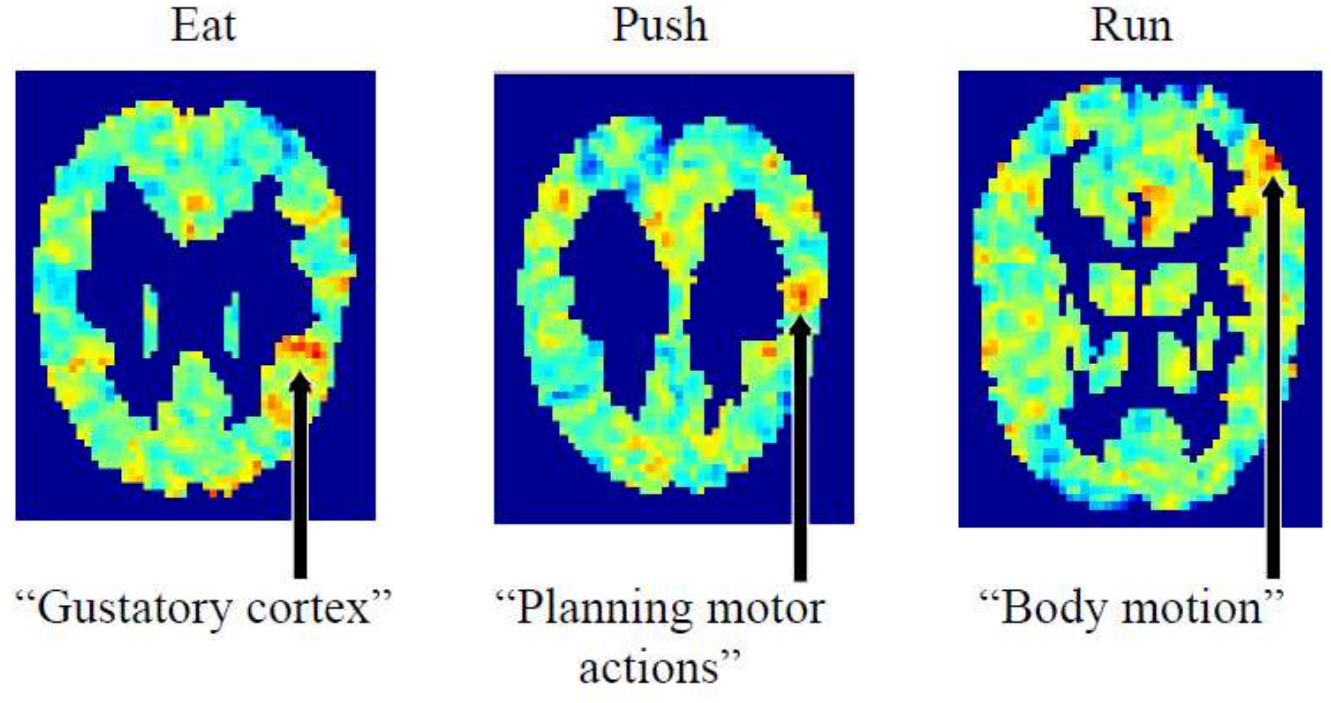
\includegraphics[width=.9\linewidth]{images/mitchell_4.png}
        \caption{The three images show the weight magnitude of each voxel, given a verb (notice different fMRI slices are shown for different verbs).}
        \label{fig:mitchell_4}
    \end{subfigure}%
    \begin{subfigure}{.47\textwidth}
        \centering
        \captionsetup{width=.8\linewidth}
        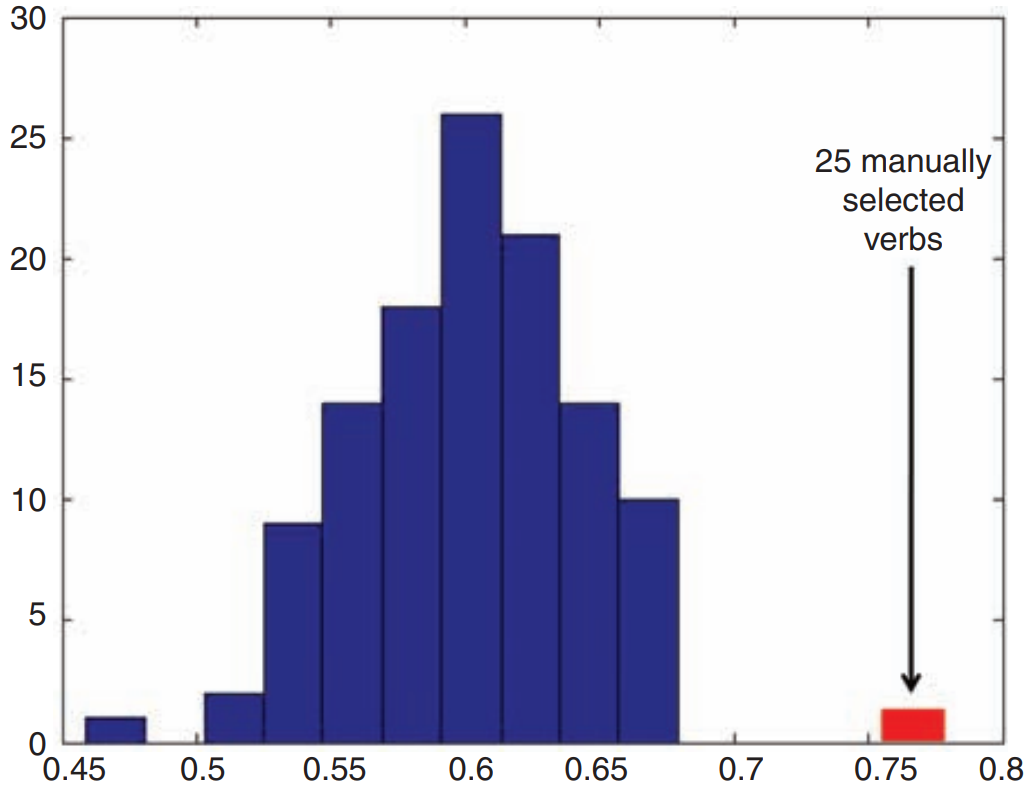
\includegraphics[width=.8\linewidth]{images/mitchell_5.png}
        \caption{Mean accuracy over 9 participants, using  randomly selected sets of intermediate semantic features vs. using the manually chosen set.}
        \label{fig:mitchell_5}
    \end{subfigure}
    \caption{Results.}
    \label{fig:mitchell_45}
\end{figure}

% \begin{figure}
%     \centering
%     \captionsetup{width=.8\linewidth}
%     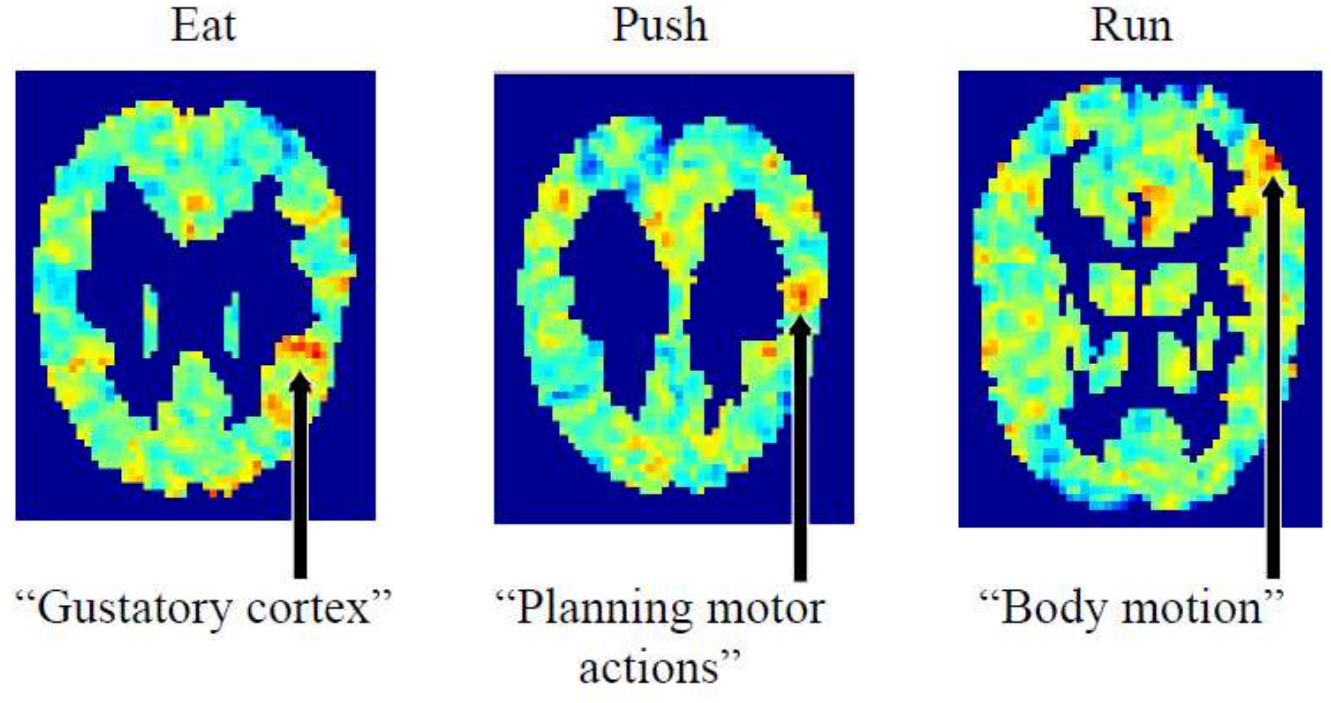
\includegraphics[width=0.5\linewidth]{images/mitchell_4.png}
%     \caption{}
%     \label{fig:mitchell_4}
% \end{figure}

Furthermore, they performed a \textit{by participant} analysis that allowed them to account for inter-individual differences. They split the brain into areas and swept through a very large number of words (10 thousands) to see \textbf{which word maximally activates that region} (or the entire brain).
They found there are indeed words that are most activating for specific brain areas.\\

In the end, they experimented with \textbf{random} \textit{25-feature-basis} sets, instead of a manually chosen set. They tried with 115 randomly selected sets (composed not only by verbs), finding that the results are much worse, yet with \textbf{significant accuracy} ($>0.61$, see Figure \ref{fig:mitchell_5}).

% \begin{figure}
%     \centering
%     \captionsetup{width=.8\linewidth}
%     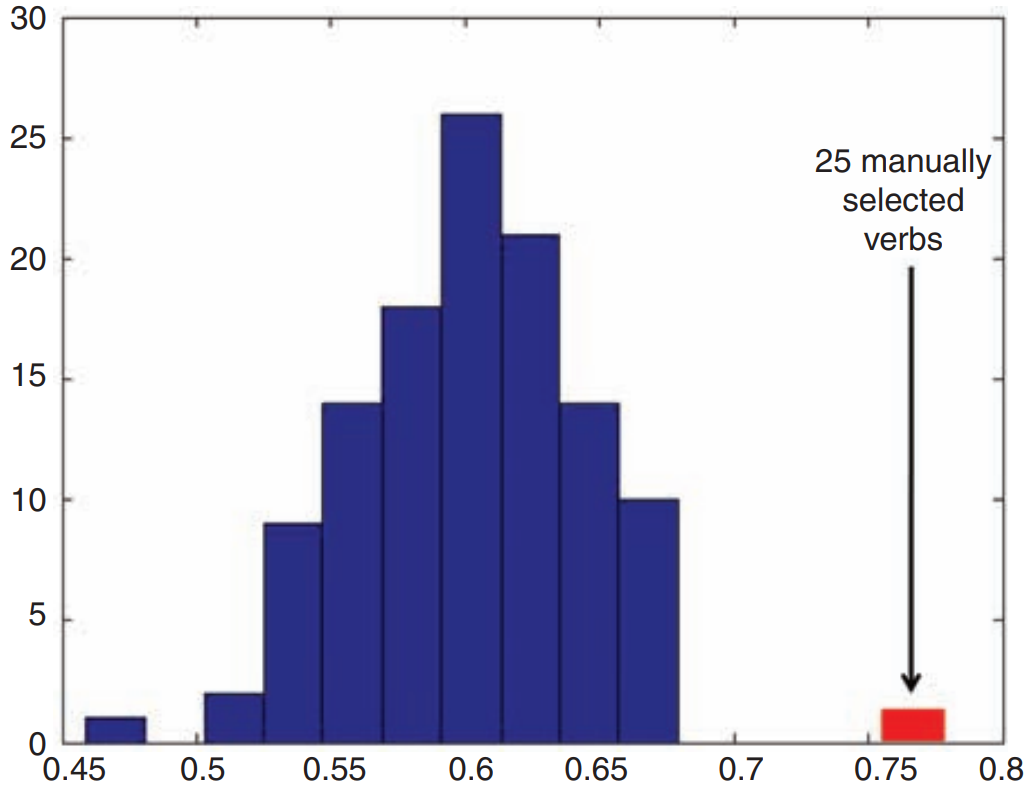
\includegraphics[width=0.45\linewidth]{images/mitchell_5.png}
%     \caption{Mean accuracy over 9 participants, using  randomly selected sets of intermediate semantic features vs. using the manually chosen set.}
%     \label{fig:mitchell_5}
% \end{figure}



\section[Studying representations via similarity spaces]{Studying representations via similarity spaces\\ \large{\textit{Matching categorical object representations in inferior temporal cortex of man and monkey}\\ Kriegeskorte et al. (2008)}}
\label{sec:kriegeskorte}
In this section we see how they model similarity spaces expressed in human behavior and brain responses.

\subsection{The principles of Representational Similarity Analysis (RSA)}
To compare if two clustering representations are similar, a possibility is to pick single elements, and check if the neighbors that are part of the same cluster in a representation, are part of the same cluster also in the other representation. This idea coming from statistics is exploited in RSA.

RSA relates modalities of human behavior (or brain activity measurement) and information processing models by \textbf{comparing activity-pattern dissimilarity matrices}. A single similarity-matrix captures \textit{first-order} similarity between stimuli (either similarity in brain response, or similarity as computed by a  model). \textbf{RSA is a 2\textsuperscript{nd} order similarity} because it quantifies how alike two similarity-matrices are.
RSA:
\begin{itemize}
    \item is modality independent: it allows to compare completely different modalities, provided we can measure similarity or distance between pairs of stimuli;
    \item can relate whatever modality of brain or behavioral  measurement to information processing models;
    \item is based on the notion of similarity, or distance, between stimuli.
\end{itemize}

\subsection{Applied contexts for RSA}

A \textbf{Representational Dissimilarity Matrix} (\textbf{RDM}) of \textbf{human behavior} is shown in Figure \ref{fig:rdm}. We can see how objects in the same category are judged to be similar (as expected). Such matrix can be populated either by directly asking pairwise similarity to people, or via item sorting tasks: given randomly placed objects, people are required to sort objects in an array with similar objects close one to each other.\\

An RDM can also be constructed on \textbf{brain data}. Figure \ref{fig:rdm_brain} shows how it is populated: we consider how much each group of voxels is related to input stimuli. We can then compare the similarity matrices as in Figure \ref{fig:rsa}.

\begin{figure}[!ht]
    \centering
    \captionsetup{width=.8\linewidth}
    \begin{subfigure}{.43\textwidth}
        \centering
        \captionsetup{width=.8\linewidth}
        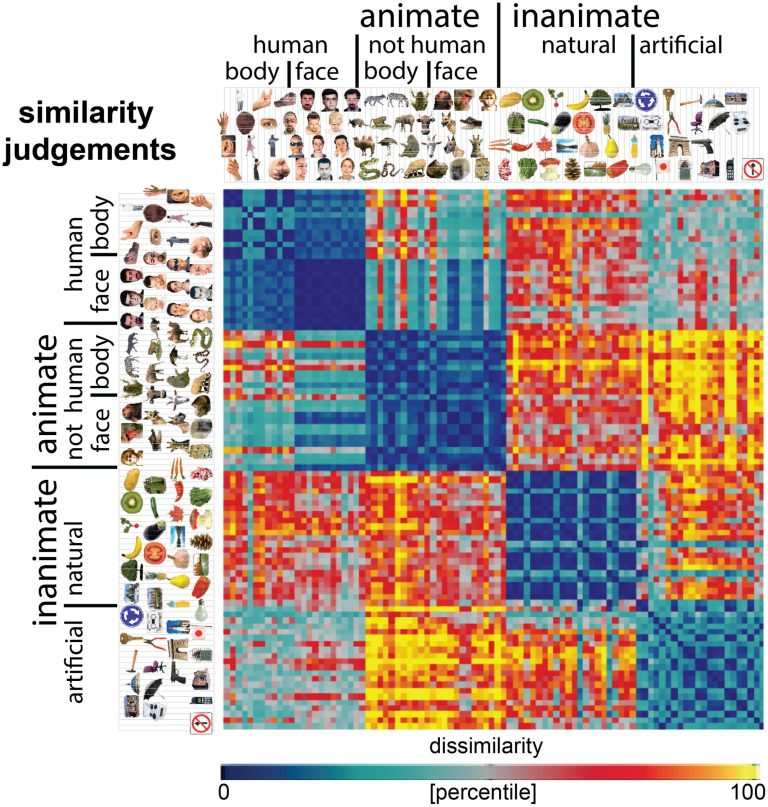
\includegraphics[width=.6\linewidth]{images/rdm.jpg}
        \caption{Example of a single RDM from human similarity judgements.}
        \label{fig:rdm}
    \end{subfigure}
    \begin{subfigure}{.54\textwidth}
        \centering
        \captionsetup{width=.8\linewidth}
        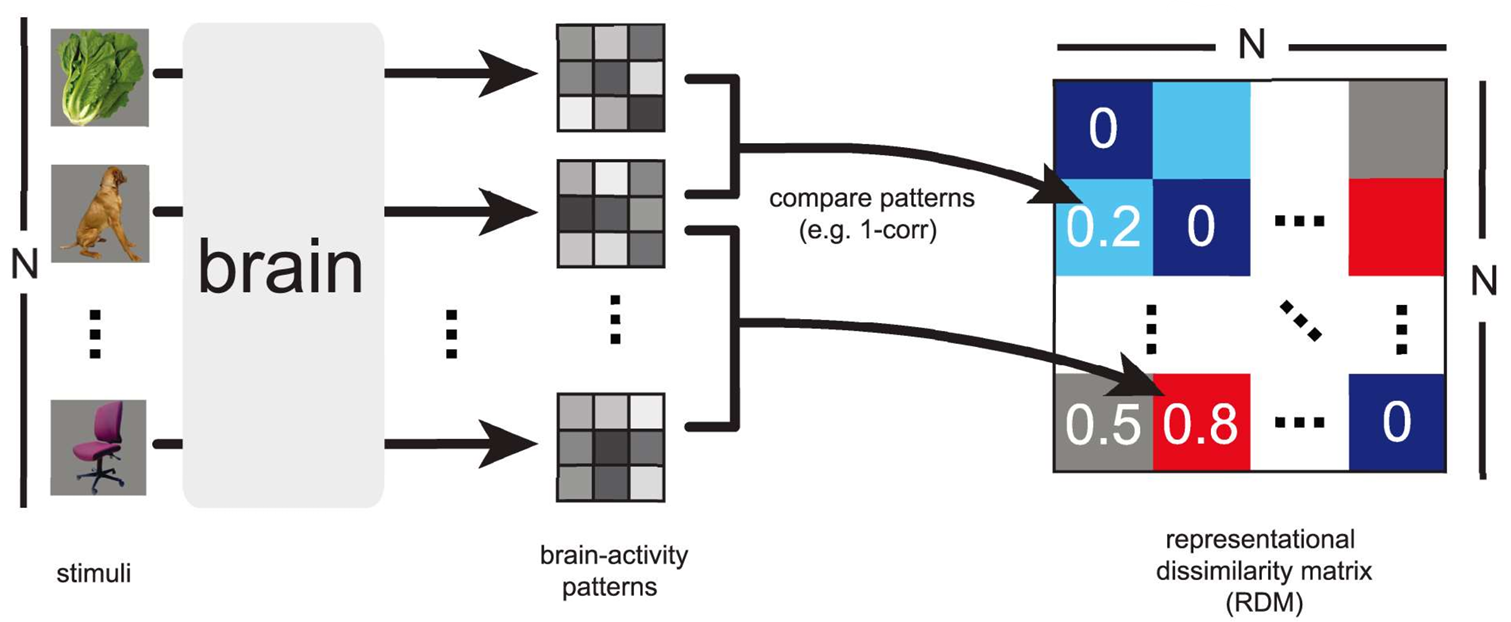
\includegraphics[width=\linewidth]{images/rdm_brain.png}
        \caption{Construction process of an RDM from brain data. For convenience, just 9 groups of voxels are represented.}
        \label{fig:rdm_brain}
    \end{subfigure}
    \caption{Examples of RDMs.}
    \label{fig:rdms}
\end{figure}

\begin{figure}[!ht]
    \centering
    \captionsetup{width=.8\linewidth}
    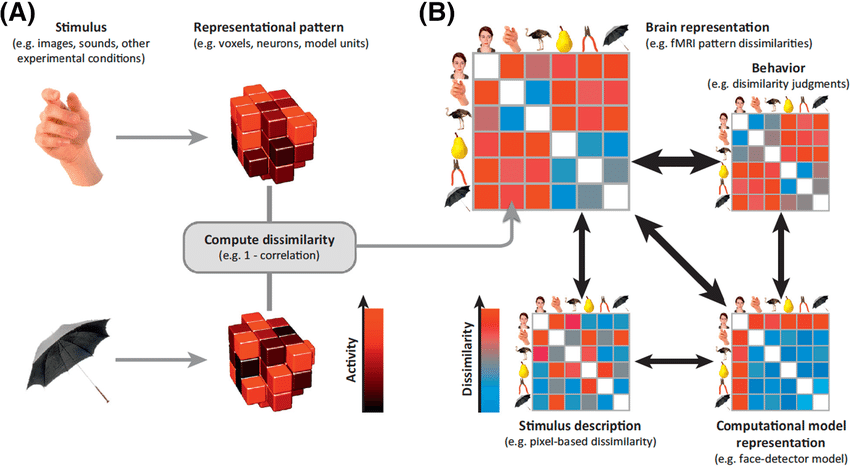
\includegraphics[width=0.7\linewidth]{images/rsa.png}
    \caption{Example of comparing RDMs, with 2 stimuli and brain response. \textbf{(A)} First-order RSA: differences between patterns of activity in a chunk of tissue responding to two objects, here a hand and an umbrella, populate one cell of an RDM in (B). \textbf{(B)} A complete RDM can now be compared using second-order RSA with other RDMs constructed from behavior, input measures, or other models.}
    \label{fig:rsa}
\end{figure}

Another possibility (Figure \ref{fig:rsa_2}) is to understand what information is coded over time, so that we can check if there is similarity between representations in the brain and in a neural network at the same depth (e.g. comparing shallow layers of the brain with shallow layers of a CNN). MEG data can be split along the time domain into intervals. For each interval, a similarity matrix is computed correlating the activity between images (note that the matrices are not the same, as representation in the brain changes over time). With fMRI data we can do another thing: relate different modalities (different brain areas), discovering that Extrastriate and Inferior temporal fit with the NN.\\

\begin{figure}[!ht]
    \centering
    \captionsetup{width=.8\linewidth}
    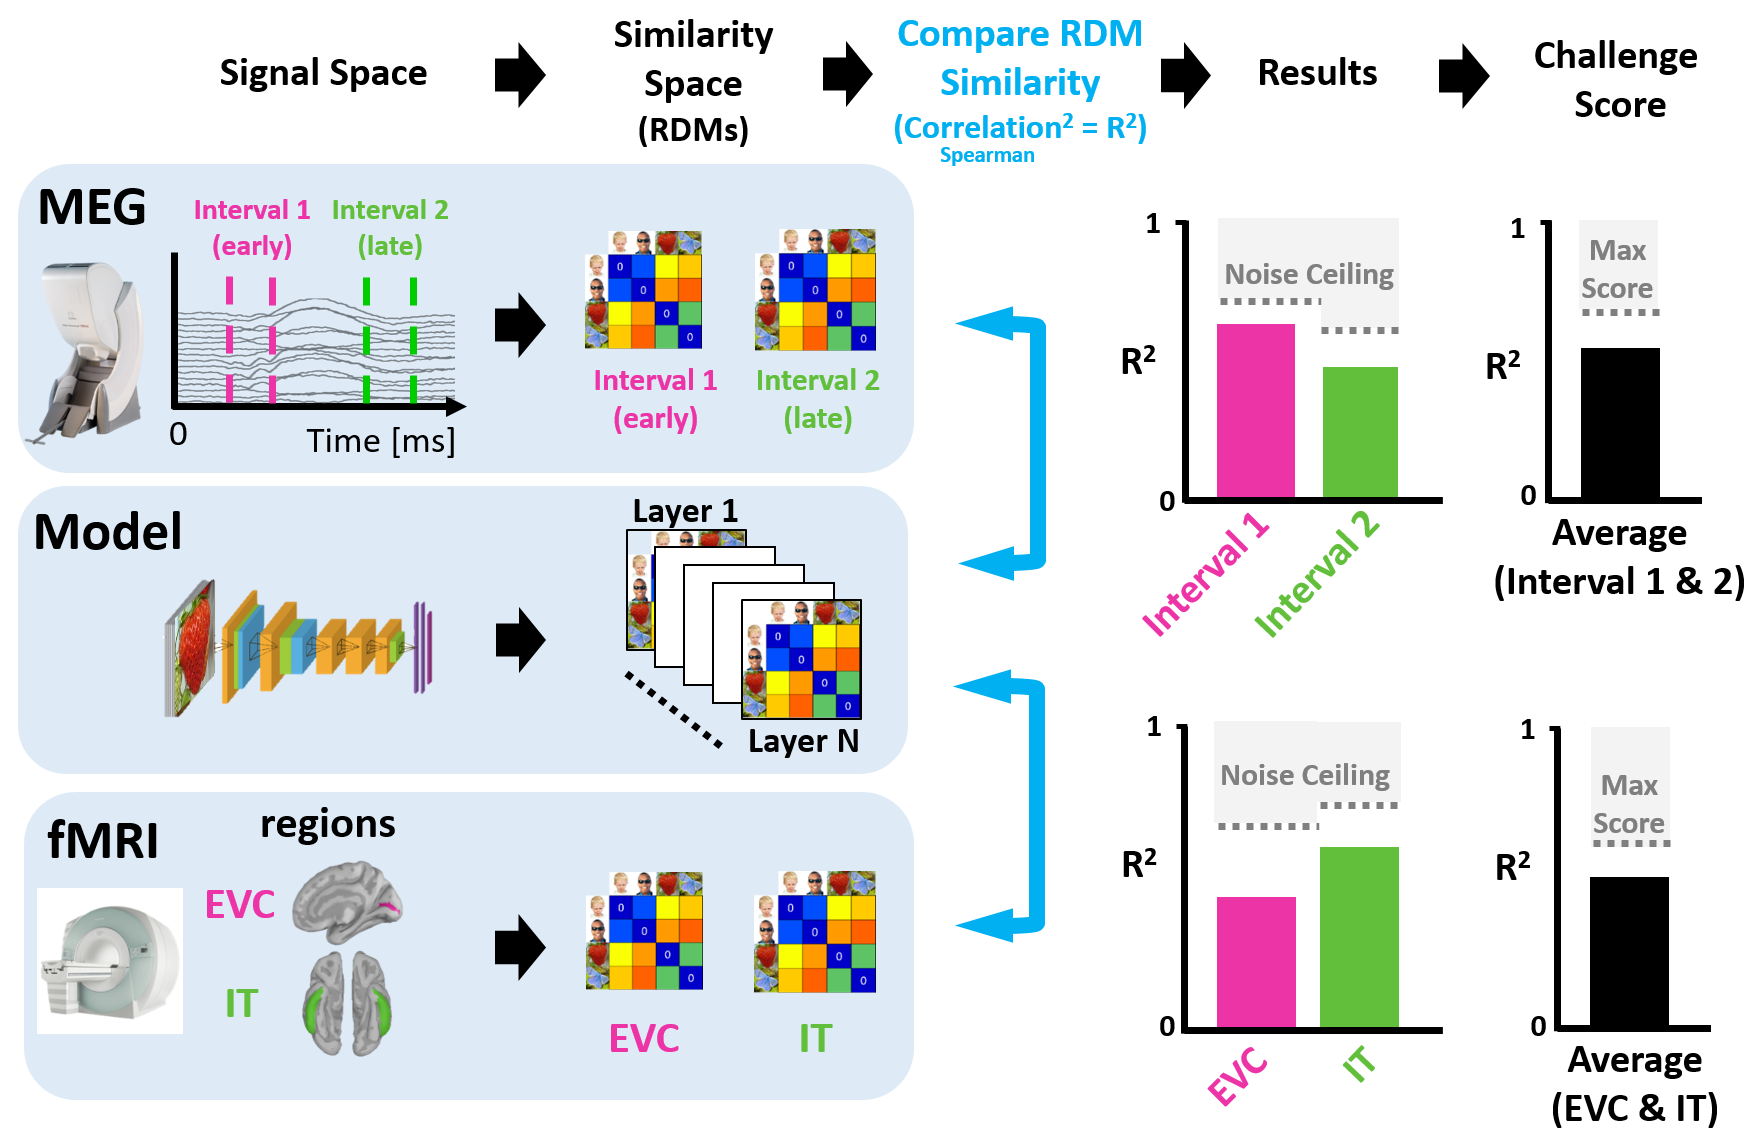
\includegraphics[width=0.7\linewidth]{images/rsa_2.png}
    \caption{Example of comparing similarity matrices. The Noise ceiling is  the maximal (ceiling) value expected given the noise in the data. Oftentimes the noise ceiling is estimated as the correlation between the estimates of the responses in two independent repetitions of the same experimental procedure. The idea is that the ability of X to predict Y cannot exceed the noise ceiling, defined as the correlation between Ys (Y1 and Y2) obtained for the same stimuli on 2 different test data.}
    \label{fig:rsa_2}
\end{figure}

Moreover, probing for 2\textsuperscript{nd} order similarity across brain regions (not against a model) allows to relate brain and behavior, find areas that code similarly for different stimuli across participants or even species. It also allows to code a single set of stimulus across multiple dimensions and code RDMs at each feature level.

\subsection{RSA and loss of dimensions}
When using Human Similarity Judgments, we create an RDM directly from those judgments (we do not have the features). 
When using NeuroBio data to produce RDMs we use an $S \times V$ (stimuli/observation $\times$ voxels/sensors/regions) matrix.
When using Computational Models to produce RDMs we use an $S \times F$ (stimuli/observation $\times$ features) matrix.
When relating NeuroBio and Computational models the [$S \times V$] and [$S \times F$] matrices are first converted to RDMs.
Consider you can get the exact same RDM from different $S \times F$ matrices that differ massively on the number of $F$. This means that when we convert to RDMs \textbf{we do not have specific information on dimensions that produce the alignment}.
\textbf{This is the main drawback of RSA}.
For instance, in the case of~\cite{Mitchell2008PredictingHB}, we get an RDM with shape [$60 \times 60$], so we lose the dimension of the 25 verbs used to compute word representations. However, the main problems of methods that keep information of the features are that they are unstable and very complicated to understand or to implement.\\

When dealing with 2 domains (brain, model) represented as observation $\times$ feature matrices, and when the two matrices reflect the same feature, we could evaluate the fit directly at the matrix level. There are many different techniques that probe for strength of common dimensions between two matrices.
\details{Digression}{
The following techniques all probe for strength of common dimensions between two matrices:
    \begin{itemize}
        \item Procrustes rotation: it takes $N$ objects in $D$ features, and tries to find a transformation to map one into the other, see image;
        \item Principal component regression (i.e., supervised PCA);
        \item Partial least squares correlation: similar to PCA, but it tries to maximize the correlation on both tables;
        \item Canonical correlation analysis.
    \end{itemize}
}

\subsection{Univariate and multivariate approaches}
In the following we consider already seen topics, but from a different perspective.

\subsubsection{Information contained in multiple voxels}
The typical approach of fMRI is massively multivariate, since it considers one voxel at a time. The problem is that information contained in multiple voxels is lost.

\begin{wrapfigure}[12]{r}{0pt}
  \centering
  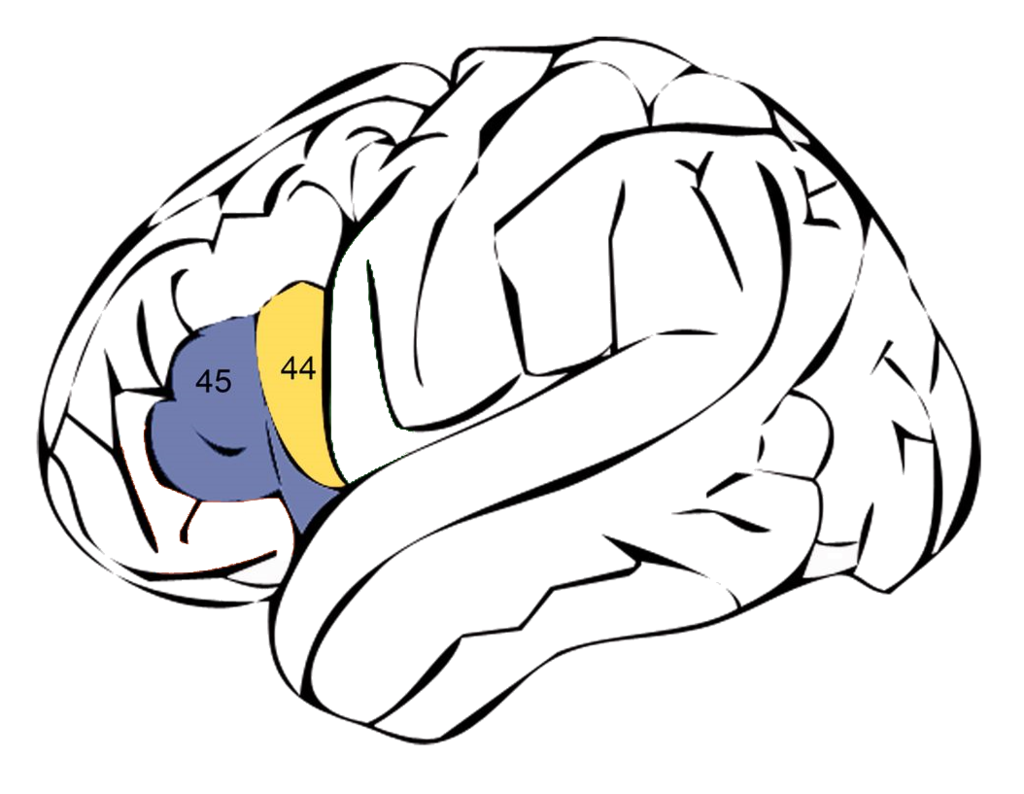
\includegraphics[width=0.23\textwidth]{images/ptri.png}
  \caption{Pars opercularis (yellow) and pars triangularis (blue).}
  \label{fig:ptri}
\end{wrapfigure}

For this reason they studied brain responses during narrative comprehension: some participants were required to focus on space, others on time, others on actions, hearing the same story.
They considered each IFG sub-region as a ``voxel".
With an univariate approach, regional activity in \textit{pars opercularis} (see Figure~\ref{fig:ptri}) was higher for some conditions, while \textit{pars triangularis} responded always with the same level of activation for the different dimensions.
In a multivariate approach, they considered the entire set of values in each region, and quantified how similar those activity patterns were for the three conditions. Instead of considering the whole area (\textit{pars triangularis}) by averaging, they kept voxels separated and found very different activations when focusing on different dimensions.

\subsubsection{Decoding category (binary case) from brain}
A multi voxel pattern analysis (MVPA) can be carried out.
Two conditions are presented, which produce different distributions of activity across trials. In Case 1, each condition produces different activity levels, in both Voxel 1 and Voxel 2. Clearly, the region discriminates the classes.
In Case 2, each condition produces highly similar mean activity levels in both Voxel 1 and Voxel 2. So one might conclude that the region does not discriminate, if aggregating across univariate analysis.
But the multivariate analysis leads to a completely different result, allowing us to better understand: the region containing voxels 1 and 2 \textbf{contains information about conditions in the joint distribution} of Voxel 1 and Voxel 2.
\begin{figure}[!ht]
    \centering
    \captionsetup{width=.8\linewidth}
    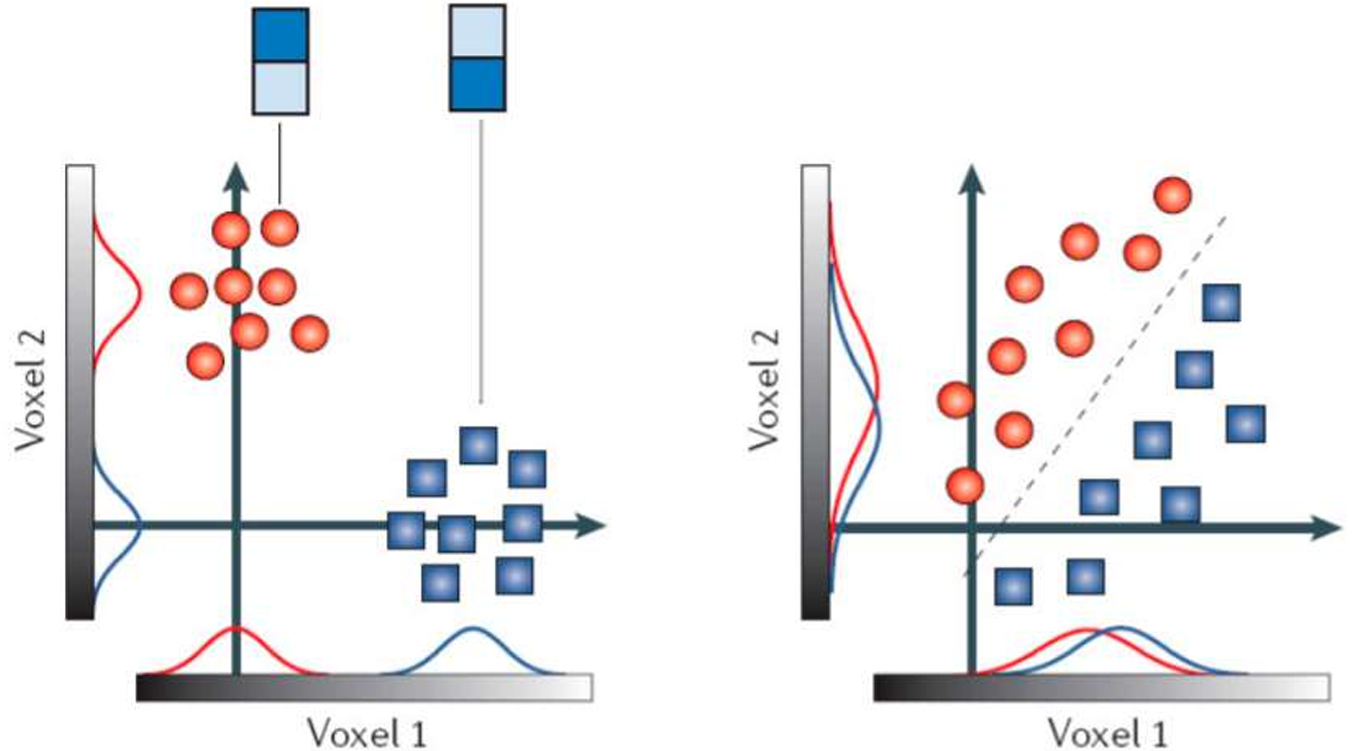
\includegraphics[width=0.5\linewidth]{images/mvpa.png}
    \caption{Case 1 on the left, Case 2 on the right. Each trial is represented as a circle or a square (depending on its category).}
    \label{fig:multivariate}
\end{figure}
